\begin{filecontents*}{example.eps}
gsave
newpath
  20 20 moveto
  20 220 lineto
  220 220 lineto
  220 20 lineto
closepath
2 setlinewidth
gsave
  .4 setgray fill
grestore
stroke
grestore
\end{filecontents*}

\RequirePackage{fix-cm}
%
%\documentclass{svjour3}                     % onecolumn (standard format)
\documentclass[smallcondensed]{svjour3}     % onecolumn (ditto)
%\documentclass[smallextended]{svjour3}       % onecolumn (second format)
%\documentclass[twocolumn]{svjour3}          % twocolumn
%
\smartqed  % flush right qed marks, e.g. at end of proof
%
\usepackage{graphicx}
%
% \usepackage{mathptmx}      % use Times fonts if available on your TeX system
%
% insert here the call for the packages your document requires
%\usepackage{latexsym}
% etc.
%
% please place your own definitions here and don't use \def but
% \newcommand{}{}
%
\usepackage{hhline}
\usepackage{natbib}
\usepackage{subfigure}
\usepackage{amssymb}
\usepackage[latin1]{inputenc}
\usepackage[usenames]{color}

% Insert the name of "your journal" with
 \journalname{Ocean Dynamics}
%
\begin{document}

\title{How to adjust tidal forcing in a fjord model
%\thanks{Grants or other notes
%about the article that should go on the front page should be
%placed here. General acknowledgments should be placed at the end of the article.}
}
%\subtitle{Do you have a subtitle?\\ If so, write it here}

%\titlerunning{Short form of title}        % if too long for running head

\author{K.~Hjelmervik \and ...
}

%\authorrunning{Short form of author list} % if too long for running head

\institute{K.~Hjelmervik \at
            University College of Southeast Norway\\
            \email{Karina.Hjelmervik@hbv.no}
            \and
            ...
}

\date{Received: date / Accepted: date}
% The correct dates will be entered by the editor


\maketitle

\begin{abstract}

Tides are one of the dominant driving forces in coastal waters. Due to complex topography with narrow and shallow straights, the tides in the innermost parts of the Norwegian fjords are both shifted in phase and altered in amplitude compared to the tides in the open water outside the fjords.

In order to model the hydrography and currents in the fjords, accurate tidal forcing is crucial. The global tidal forcing is too coarse for fjord modeling since tides vary over short distances close to the coast line. Therefore, the tidal forcing has to be adjusted to fit the actual tides in the area. We have developed a simple method to do this adjustment. First, a high-resolution ocean model is run with the global tidal forcing on the open boundary. Time series of water level is then analysed and compared with observed water level. Based on the comparison a factor for the amplitude and a phase shift is computed and applied to produce adjusted tidal forcing. The same factor and phase shift is used on tidal current forcing as for tidal water level forcing. The model is then rerun with the adjusted tidal forcing.

The method is tested in the Regional Ocean Model System (ROMS) on two different model areas in Norway; Oslo fjord and Saltstraumen. The results show a promising improvement in modelled tides in both the inner and the outer parts of the fjords. 

\end{abstract}

\section{Introduction}

Tides are one of the dominant contributor to sea level variations along the Norwegian coast \cite[]{grabbe09}. The exception are storm surge events \cite[]{lynge13}.

The tides are one of the major driving forces in the fjords. \textcolor{Red}{Noe generelt om fjordmodeller}

The tides are often imposed only on the boundary of the fjord models. Close to the coastline, the tides vary over short distances. The TPXO Atlantic database with a horizontal resolution of 1/30$^o$ \cite[]{egbert94,egbert02} is too coarse to get the correct phase and amplitude. Here we propose a new method on how to adjust the global tidal forcing to local ocean models. 

\section{Area of interest}
Two areas are chosen in this study in order to investigate if the method handles different types of fjords.

\begin{figure}[!t]
\centering
\includegraphics[width=0.5\textwidth]{fig_Oslofjorden_area}
\caption{The Oslo fjord. The position of the four tide gauges in Oslo, Oscarsborg, Viker, and Helgeroa are marked.}
\label{fig:area1}
\end{figure}

The Oslo fjord is located in the southeastern part of Norway with the main city of Norway in the innermost part of the fjord (Fig.~\ref{fig:area1}). The fjord lies in the most populated area of Norway and it is therefore important to gain knowledge on this fjord. The fjord has an interesting flow pattern due to several river outlets, thresholds, complex topography, storm situations in Skagerak, and atmospheric forcing.
Even though the mean total tidal elevation is less than 20 cm in the Oslo fjord, the tidal currents are up to 0.5 m/s due to the narrow straits and thresholds.In connection with storm surge events, a maximum amplitude of 70 cm is observed. The Oslo fjord has an open, southern boundary towards Skagerak which lies in the eastern part of the North Sea. The circulation in the Skagerak is anticlockwise with brackish outflow from the Baltic Sea \cite[]{rodhe96,svendsen96}. 


\begin{figure}[!t]
\centering
\includegraphics[width=0.8\textwidth]{fig_Saltstraumen_area}
\caption{The Saltstraumen is a strong current in a narrow passage between the Salt fjord and the Skjerstrad fjord. The position of the tide gauge in Bod\o is marked.}
\label{fig:area2}
\end{figure}

The Saltfjord is located in the northern part of Norway (Fig.~\ref{fig:area2}). Saltstraumen is a small straight at the entrance of the Skjerstad fjord and is counted as the world's strongest tidal currents. The difference between the water level before the narrow straight and after the narrow straight can be up to one meter, causing water speeds up to 11 m/s \cite[]{eliassen01}.

The inner part of the fjord system, the Skjerstad fjord, is a deep glacially carved basin separated from the outer part, the Salt fjord, by a sill in the narrow current named Saltstraumen. This fjord system is generally deep, but the depth from the sill to the mouth of Saltfjorden is less than the depth of the inner part, Skjerstadfjorden. The sill in Saltstraumen is about 50 km from the head of the fjord system. The sill depth is 26 m and the depth in the basin inside the sill is more than 500 m: The inner basin and the sill area are connected by a channel which is much deeper and a little wider than Saltstraumen.

The Norwegian Mapping Authority, Hydrographic Service has 23 tide gauges along the Norwegian coast included one at Spitsbergen. Data is available from 1992 up to the current year. Four of the gauges are placed in the Oslofjord  (Fig.~\ref{fig:area1}) and one close to the open boundary of the Salt fjord (Fig.~\ref{fig:area2}).


\section{Model setup}

The Regional Ocean Model System (ROMS) version 3.6 is applied for both fjords as described in \cite{roed16}. ROMS is a free-surface, terrain-following, primitive equations ocean model widely used by the scientific community for a diverse range of applications \cite[]{shchepetkin05,shchepetkin09,haidvogel08}. 

The fjord models are nested into the NorKyst800 model \cite[]{albretsen11} through daily means. \textcolor{Red}{[}The NorKyst800 model covers the whole Norwegian coast with a resolution of 800 meters. Despite NorKyst800s relatively high resolution it is still not fine enough to resolve the highly irregular geometry and topography of most Norwegian fjords (see Fig.~\ref{fig:NorKyst}). - \textcolor{Red}{fjernes?]}

For both fjords high-resolution, curvilinear grids are applied with 42 terrain-following layers in the vertical using a continuous, double stretching function following \cite{shchepetkin09}. Water levels less than two meters are set to zero. Thereby the shallow parts of the fjords are omitted. In order to avoid model instability and/or spurious deep currents the final masked bathymetry is smoothed as described in \cite{roed16}.

%In the horizontal a curvilinear grid with varying grid size is applied (Fig.~\ref{fig:GridSize}). The characteristic grid size, $\Delta s_{i,j}$, is taken as:
%\begin{eqnarray}
%\Delta s_{i,j}^2 \! = \! 
%\left(\!(x_{i+1,j}-x_{i,j})^2\!\! + \!(y_{i+1,j}-y{i,j})^2\! \right)^{\!0.5}\!\!
%\left(\!(x_{i,j+1}-x_{i,j})^2\!\! + \!(y_{i,j+1}-y_{i,j})^2\! \right)^{\!0.5}
%\end{eqnarray}
%Here $i = 1, \cdots, 299$ and $j =1, \cdots, 899$. $x_{i,j}$ and $y_{i,j}$ are the rho-coordinates of element $(i,j)$. (Sp\o rsm\aa l: Er det hensiktsmessig \aa ta med dette?)

%\begin{figure}[!t]
%\centering
%%\includegraphics[width=0.4\textwidth]{Figurer/GridSize}
%\caption{Characteristic grid size in the whole model area.}
%\label{fig:GridSize}
%\end{figure}

\begin{figure}[!t]
\centering
%\includegraphics[width=0.4\textwidth]{Figurer/GridSize}
\caption{NorKyst area \textcolor{Red}{- fjernes?}}
\label{fig:NorKyst}
\end{figure}

The necessary atmospheric input (wind, pressure, temperature, humidity, and cloud cover) is extracted from the AROME-MetCoOp model with a grid resolution of 2.5 km \cite[]{muller2015}. The freshwater discharges to are taken data from a database constructed by use of the hydrological model HBV \cite[]{beldring2003}.

The tidal input in terms of tidal elevations and currents are based on the TPXO Atlantic database \cite[]{egbert02} for the Oslofjord model. Due to technicalities the TPXO 7.2 were applied for the Saltfjord model. The tidal forcing is to coarse for fjord modeling since the tides vary over short distances and a simple interpolation to the model grid might not be sufficient close to the coast line. In order to omit this problem, other fjord models applies tidal amplitude and phase from observed water level close to the boundary \cite[i.e.]{svendsen96,lynge13}. In the ROMS model it is preferable to include the tidal current major amplitude, minor amplitude, phase, and inclination angle. Here we propose a method on how to adjust the global tidal forcing in terms of both elevation and currents, to local ocean models. 

\section{Method}

The method is straight forward. First the tidal forcing, the Atlantic TPXO with a resolution of 1/30 degree for the Oslofjord model and the TPXO 7.2 with a resolution of 1/4 degree for the Saltfjord model, were imposed at the open boundaries of the fjord models. The simulated time period is 180 days. 

Time series of observed and simulated water level from locations close to the tidal gauge stations close to the open boundaries, were extracted and analysed based on the T\_Tide package described by \cite{pawlowicz02}. For the Oslofjord model, observed and modelled water level are extracted from a location near Viker which lies inside the model domain. For the Saltfjord model, observed and modelled water level are extracted from a location near Bod\o which lies slightly outside the model domain. Ten major tide constitutents of diurnal (K$_1$, P$_1$, and O$_1$), semidiurnal (K$_2$, S$_2$, M$_2$, and N$_2$), and quarter-diurnal (MN$_4$, M$_4$, and MS$_4$) frequencies are retrieved from the observed and modelled time series. 

To better match the observations, the tidal amplitudes and corresponding phase were modified by computing an amplitude factor, $c^{(n)}$, and a phase shift, $\triangle \phi^{(n)}$, for each tidal component $n$ for the water level according to:
\begin{eqnarray}
c^{(n)} &=& \frac{a^{(n)}_{obs}}{a^{(n)}_{sim}} \\
\triangle \phi^{(n)} &=& \phi^{(n)}_{obs} - \phi^{(n)}_{sim}
\end{eqnarray}
$a^{(n)}_{obs}$ and $a{(n)}_{sim}$ are the observed and simulated amplitude respectively. $\phi^{(n)}_{obs}$ and $\phi^{(n)}_{sim}$ are the observed and simulated phase respectively.. 

New amplitudes and phases at the boundary were then calculated using the computed factors and phase shifts on both water level and velocity. The new amplitudes and phases imposed at the open boundaries of new simulations where taken as:
\begin{eqnarray}
a^{(n)}_{i2} &=& a^{(n)}_{i1} c^{(n)} \\
\phi^{(n)}_{i2} &=& \phi^{(n)}_{i1} + \triangle \phi^{(n)}
\end{eqnarray}
$a^{(n)}_{i1}$ and $\phi^{(n)}_{i1}$ are the amplitude and phase originally imposed on grid cell $i$ along the boundary. Modified major and minor amplitude and phase for the tidal current are adjusted in the same way using the amplitude factor and phase shift calculated from the water level. The inclination angles are not adjusted.

The models are then rerun with the adjusted tidal forcing. The results are then analysed as for the first run and  compared with observed tidal water level. 

\section{Discussion and results}

\textcolor{Red}{Her er det mye rot. Arbeider med � rydde. Karina}

Here is the observed tidal water level in red and the simulated tidal water level in black. As you can see the amplitudes are not correct and also the phase is a little bit off.

Nine tidal constitutes are included in the tidal forcing. As you can see the difference in observed and simulated amplitude for M2 is 2 cm and the phase difference 12 degrees. Based on that we calculate the ratio and the phase difference, and apply it on the tidal forcing.

We then rerun the model with adjusted tidal forcing, do the harmonic analyses and compare again with the observed time series. Here we have plotted the combined tidal amplitudes of the nine components.  And as you can see the results are pretty descent. 

Here are the tidal amplitudes for the nine components in three different positions were we have permanent tidal gauges. We do not have a perfect match, but the results are promising. 

The spatial variation is larger in the Salt fjord. The Saltstraumen is one of the worlds strongest tidal currents. Due to a narrow passage the tidal amplitude is much smaller inside the narrow passage than outside the passage, resulting in strong currents. 

The model is run twice. First with the original tidal forcing. Secondly with the adjusted tidal forcing. Table \ref{tab:Viker} shows that the adjustment has the desired effect close to the open boundary. Table \ref{tab:Oscarsborg} shows that the simulated tides are distributed as intended in the inner parts of the fjord.

The tidal current components vary across the fjord.... \cite{lynge13}.

The resulting new tidal amplitudes and periods for the locations close to the Viker and Oscarsborg tidal gauge stations are shown in Tables 3 and 4 in column Modified. The results are clearly improved at both stations. In particular we are pleased with the results close to the Oscarsborg tidal gauge station which may be viewed as a control station in that it is far away from the southern boundary where the tidal forcing is imposed.

Fields of the amplitude and phase for M$_2$ reveal som interesting phenomenas (Figure \ref{fig:Oslofjord_tidal_fields}). North of the western branch of the Oslo fjord the amplitude decreases as the water has to pass through a very narrow passage called Svelvikstraumen. North of the eastern branch the amplitude increases. The phase is more delayed north of the eastern branch than the western branch. The observed phase delay is more pronounced in the observations than the model. \textcolor{Red}{B{\o}r sette inn noen tall fra tabellene}


\begin{figure}[!t]
\centering
\includegraphics[trim=1cm 1cm 0cm 0cm,clip=true,width=0.49\textwidth]{fig_Oslofjorden_M2amp.eps}
\includegraphics[trim=1cm 1cm 0cm 0cm,clip=true,width=0.49\textwidth]{fig_Oslofjorden_M2phase.eps}
%\includegraphics[width=0.33\textwidth]{fig_Oslofjorden_M2camp.eps}
\caption{Fields of M$_2$ water level amplitude and phase in the Oslo fjord. The corresponding observed values are indicated by colored cirles at the three permanent gauges in the area.}
\label{fig:Oslofjord_tidal_fields}
\end{figure}

\begin{table}[ht]
%\vspace{-1.5cm}
\caption{Tidal amplitudes [cm] and phases [deg] for the water level at Viker. \textcolor{Red}{M{a} oppdateres!}}
\label{tab:Viker}
\centering
\begin{tabular}{@{}c@{$\;\;$}r@{$\;\;$}r@{$\;\pm\;$}rr@{$\;\pm\;$}rr@{$\;\pm\;$}rr@{$\;\pm\;$}rr@{$\;\pm\;$}rr@{$\;\pm\;$}r} \hline
      & Period & \multicolumn{4}{c}{Observed} & \multicolumn{4}{c}{Run 1} & \multicolumn{4}{c}{Run 2} \\
Comp. & [h] $\;\;$ & \multicolumn{2}{c}{[cm]} & \multicolumn{2}{c}{[deg]} & \multicolumn{2}{c}{[cm]} & \multicolumn{2}{c}{[deg]} & \multicolumn{2}{c}{[cm]} & \multicolumn{2}{c}{[deg]} \\ \hline 
S$_2$   & 12.0000 &  2.3 &  0.7 &   48 &   15 &  5.1 &  1.0 &   81 &   11 &  3.2 &  0.3 &   67 &    5 \\ 
M$_2$   & 12.4206 & 12.4 &  0.7 &  115 &    3 &  9.7 &  1.1 &  122 &    6 & 11.8 &  0.3 &  105 &    1 \\ 
N$_2$   & 12.6583 &  2.8 &  0.7 &   69 &   14 &  5.7 &  1.1 &   81 &   11 &  3.1 &  0.3 &   69 &    5 \\ 
K$_1$   & 23.9345 &  0.7 &  0.6 &   98 &   49 &  1.2 &  0.5 &  212 &   23 &  0.1 &  0.1 &  198 &   97 \\ 
O$_1$   & 25.8193 &  2.1 &  0.7 &  282 &   20 &  3.7 &  0.4 &   19 &    8 &  2.9 &  0.2 &  338 &    3 \\ 
Q$_1$   & 26.8684 &  1.0 &  0.6 &  221 &   42 &  0.1 &  0.3 &  215 &  154 &  0.1 &  0.1 &  253 &  156 \\ 
MN$_4$  &  6.2692 &  0.4 &  0.2 &  270 &   24 &  1.0 &  0.2 &  141 &   12 &  0.3 &  0.0 &    7 &    3 \\ 
M$_4$   &  6.2103 &  1.4 &  0.2 &  287 &    7 &  0.7 &  0.2 &   25 &   17 &  1.1 &  0.0 &  354 &    1 \\ 
MS$_4$  &  6.1033 &  0.4 &  0.2 &    5 &   28 &  1.1 &  0.2 &  111 &   12 &  0.6 &  0.0 &   80 &    1 \\ 
\hline
\end{tabular}
\end{table}

\begin{table}[ht]
%\vspace{-1.5cm}
\caption{Tidal amplitudes [cm] and phases [deg] for the water level at Oscarsborg. \textcolor{Red}{M{a} oppdateres!}}
\label{tab:Oscarsborg}
\centering
\begin{tabular}{@{}c@{$\;\;$}r@{$\;\;$}r@{$\;\pm\;$}rr@{$\;\pm\;$}rr@{$\;\pm\;$}rr@{$\;\pm\;$}rr@{$\;\pm\;$}rr@{$\;\pm\;$}r} \hline
      & Period & \multicolumn{4}{c}{Observed} & \multicolumn{4}{c}{Run 1} & \multicolumn{4}{c}{Run 2} \\
Comp. & [h] $\;\;$ & \multicolumn{2}{c}{[cm]} & \multicolumn{2}{c}{[deg]} & \multicolumn{2}{c}{[cm]} & \multicolumn{2}{c}{[deg]} & \multicolumn{2}{c}{[cm]} & \multicolumn{2}{c}{[deg]} \\ \hline 
S$_2$  & 12.0000 &  2.7 &  0.8 &   70 &   18 &  6.1 &  1.3 &   85 &   11 &  3.7 &  0.4 &   70 &    7 \\ 
M$_2$   & 12.4206 & 14.1 &  0.7 &  132 &    3 & 11.1 &  1.2 &  128 &    7 & 13.7 &  0.3 &  111 &    2 \\ 
N$_2$   & 12.6583 &  3.0 &  0.8 &   85 &   15 &  6.6 &  1.4 &   86 &   10 &  3.6 &  0.4 &   75 &    6 \\ 
K$_1$   & 23.9345 &  1.2 &  0.5 &  101 &   35 &  1.1 &  0.5 &  213 &   27 &  0.1 &  0.2 &   44 &   79 \\ 
O$_1$   & 25.8193 &  2.1 &  0.7 &  286 &   17 &  3.9 &  0.5 &   21 &    8 &  3.1 &  0.2 &  340 &    4 \\ 
Q$_1$   & 26.8684 &  1.0 &  0.7 &  230 &   36 &  0.2 &  0.4 &  204 &  126 &  0.0 &  0.2 &  190 &  165 \\ 
MN$_4$  &  6.2692 &  0.6 &  0.3 &  316 &   26 &  2.0 &  0.4 &  163 &   14 &  0.5 &  0.0 &   29 &    3 \\ 
M$_4$   &  6.2103 &  2.1 &  0.3 &  332 &    8 &  1.4 &  0.4 &   44 &   19 &  2.0 &  0.0 &   14 &    1 \\ 
MS$_4$  &  6.1033 &  0.5 &  0.3 &   57 &   32 &  2.2 &  0.4 &  135 &   11 &  1.3 &  0.0 &  106 &    1 \\ 
\hline
\end{tabular}
\end{table}

The presence of Saltstraumen as a major impact on the circulation in the Salt fjord. According to \cite{svendsen96} an anticyclonic vortex is formed to the northeast of Saltstraumen, and a cyclonic vortex to the northwest.
% Fra Svendsen et. al 1996
%They are caused by the high velocity water coming out from Saltstraumen on the falling tide, where the velocity reaches a maximum of about 4 m s1: The anti-cyclonic vortex is weaker when the tide is rising, but does not reverse direction. The cyclonic vortex almost vanishes on rising tides. These results are in accordance with the results from Resipientunderskelse (Anon., 1990) where a direct measurement of the velocity field was performed over a time period of 10 days.

The modelled water level at Bod{\o} from the run with TPXO 7.2 applied as tidal forcing, the tidal amplitudes were too small and the phase was shifted forward in time (Figure \ref{fig:Saltstraumen_timeseries}). The adjustment factor and phase shift was computed for every tidal component based on harmonic analyses and the adjusted tidal forcing was computed. When the model was rerun, the modelled water level at Bod{\o} was more similar to the observations, but still too small. The error in phase for M$_2$ was only 0.8 degrees which corresponds to three minutes (Table \ref{tab:Bodo}).

\begin{figure}[!t]
\centering
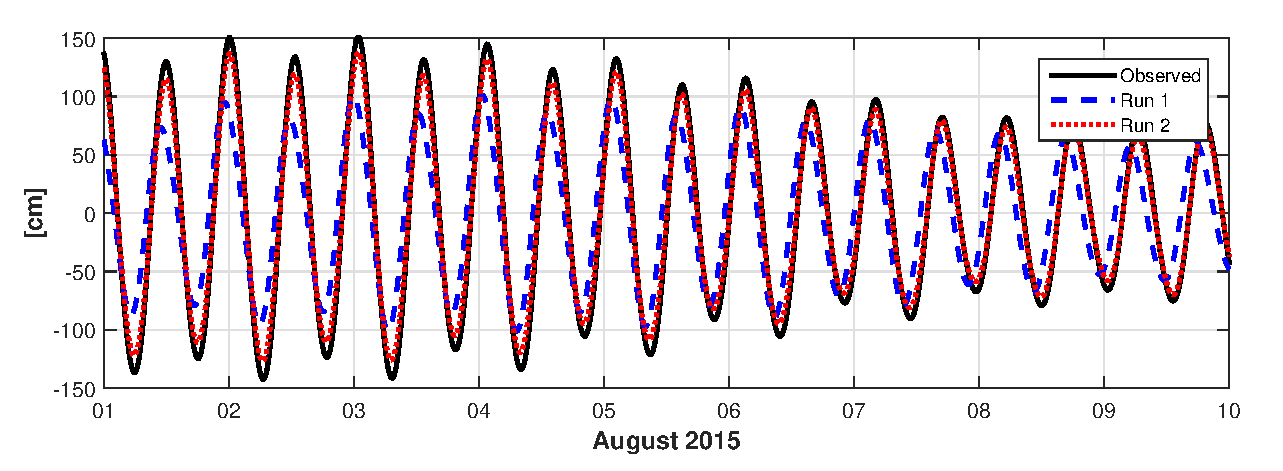
\includegraphics[width=\textwidth]{fig_Saltstraumen_timeseries}
\caption{Time series of water level at a position close to Bod\o}
\label{fig:Saltstraumen_timeseries}
\end{figure}


\begin{figure}[!t]
\centering
\includegraphics[width=\textwidth]{fig_Saltstraumen_M2amp}
\includegraphics[width=\textwidth]{fig_Saltstraumen_M2phase}
\caption{Fields of M$_2$ water level amplitude and phase in the Salt and Skjerstad fjords.}
\label{fig:Saltstraumen_field}
\end{figure}

\begin{table}[ht]
%\vspace{-1.5cm}
\caption{Tidal amplitudes [cm] and phases [deg] for the water level at Bod{\o} together with adjustment factor $c$ and phase shift $\triangle \phi$ for each component}
\label{tab:Bodo}
\centering
\begin{tabular}{crrrrrrrrrr} \hline
      & Period & \multicolumn{2}{c}{Observed} & \multicolumn{2}{c}{Run 1} & \multicolumn{2}{c}{Run 2} & \multicolumn{2}{c}{Adjustment} \\
Comp. & [h] $\;\;$ & [cm] & [deg] & [cm] & [deg] & [cm] & [deg] & $c\;\;$ & $\triangle \phi$  \\ \hline 
S$_2$   & 12.0000  &  30.0 &      8   &  19.1 &     16   &  28.1 &      7    &   1.570  &    -7.2   \\ 
M$_2$   & 12.4206  &  87.3 &    331   &  60.0 &    301   &  78.3 &    330    &   1.454  &    29.8   \\ 
N$_2$   & 12.6584  &  18.5 &    308   &  12.7 &    271   &  16.7 &    309    &   1.461  &    37.2   \\ 
K$_1$   & 23.9345  &  10.8 &    194   &   8.8 &    183   &  10.7 &    194    &   1.225  &    11.5   \\ 
O$_1$   & 25.8193  &   3.8 &     33   &   3.3 &     39   &   3.7 &     33    &   1.154  &    -6.1   \\ 
MN$_4$  &  6.2692  &   1.5 &    229   &   0.4 &    122   &   1.5 &    228    &   3.000  &   106.9   \\ 
M$_4$   &  6.2103  &   2.7 &    268   &   3.3 &    159   &   3.1 &    283    &   0.808  &   109.5   \\ 
MS$_4$  &  6.1033  &   1.3 &      2   &   1.5 &    152   &   1.4 &     30    &   0.861  &  -149.6   \\ \hline
\end{tabular}
\end{table}


\section{Conclusion}

\textcolor{Red}{Skrives til sist}

Accurate tidal forcing is important in fjord models...

We have proposed a new and simple method to adjust tidal forcing. The method is straight forward. First we run the ocean model with global tidal forcing, for example the global TPXO with a resolution of 1/4 degree. Secondly, we run harmonic analysis in order to compare the simulated and observed water level for each tidal component. The ratio between observed and simulated amplitude and a phase difference are computed for each tidal component. The ratio and the phase difference are used to adjust the tidal forcing. The same ratio and phase difference is applied on the amplitudes of both water level and current. The model is rerun with adjusted tidal forcing and the results checked.

The method is tested on two different areas, the Oslofjord and the Saltfjord, both in Norway.
 
The results are promising 

\bibliographystyle{apalike}
\bibliography{Bibliography_Tide}

\end{document}
